\section{Post-simulation analysis}
CpHMD simulations allow the user to determine
the protonation states of all titratable sites
at the simulation pH conditions, 
the {\pka} values, 
or pH- or proton-coupled conformational dynamics. 
Below we will discuss these aspects. 

\subsection{Determination of protonation states and {\pka} values}
The lambda file contains the time evolution of $\lambda$ (titration state) 
and $x$ (tautomeric state) coordinates of titratable groups.
These data allow us to determine the protonation
states at specific pH, calculate the
{\pka} values and tautomer states, and 
monitor convergence of protonation-state sampling.
As an example, Fig.~\ref{Fig:lambda_time} shows the time evolution 
of $\lambda$ for Cys481 in the BTK kinase
at different pH conditions.

 %--------------------------------------------- 
\begin{figure}[htb!]
    \centering
    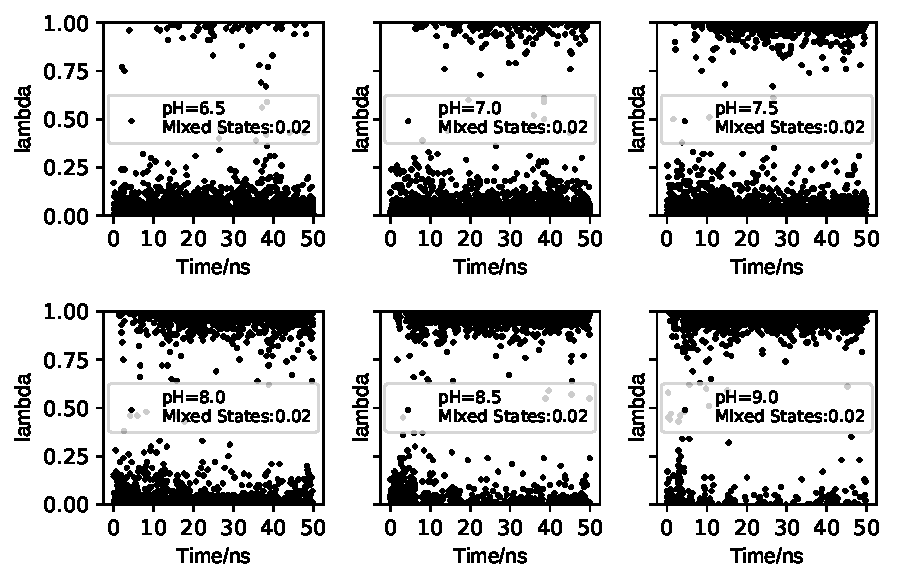
\includegraphics[width=3.6in]{figs/btk_c481_lambdavstime.pdf}
    \caption{\textbf{Time series of the $\lambda$ value for Cys481 in the BTK kinase.} 
    The data were saved every 20 ps (taken from Ref \cite{Liu_Shen_2021_J.Med.Chem.}). 
    The pH conditions and fractions of mixed states ($0.2 \le \lambda \le 0.8$) are given. 
    The plots show that the protonation-state sampling at all pH conditions 
    converge after $\sim$10 ns.
    }
\label{Fig:lambda_time}
\end{figure}
 %--------------------------------------------- 
 
To facilitate analysis of the lambda files, we developed a Python tool \href{https://gitlab.com/shenlab-amber-cphmd/cphmd-analysis}{cphmd\_anal.py}. 
This tool returns plots of the time series of unprotonated fractions and 
fitting of the unprotonated fractions to obtain {\pka's} (see discussion below).
For a trajectory at a specific pH, 
we can count the number of frames where a titratable residue $i$ is 
in the protonated or unprotonated state, which is defined 
as $\lambda_i < 0.2$ or $\lambda_i > 0.8$, respectively.
The unprotonated fraction of the residue ($S_i$)
is calculated as
\begin{equation}
S_i = \frac{N_i^{\rm Unprot}}{N_i^{\rm Prot} + N_i^{\rm Unprot}},
\end{equation}
where $N_i^{\rm Prot}$ and $N_i^{\rm Unprot}$ are
the number of protonated and unprotonated frames,
respectively.
Plotting the time series of the $S_i$ value informs
convergence of the protonation state sampling (Fig.~\ref{fig:intro}, step 5).
Once convergence is reached, the {\pka} of residue $i$
can be obtained by fitting the $S_i$ 
values at all simulation pH to 
the generalized Henderson-Hasselbalch equation,
\begin{equation}
S_i = \frac{1}{1+10^{n(\rm pK_{a,i} - pH)}},
\end{equation}
where $n$ is the Hill coefficient.
The resulting best fit is referred to as the titration curve (Fig.~\ref{fig:intro}, step 5).
A significant deviation of $n$ from 1 indicates cooperativity
($n>1$)
or anti-cooperativity ($n<1$) with a neighboring residue.
We note, in the past, $\lambda_i < 0.1$ and $\lambda_i > 0.9$ were used for
defining the protonated and unprotonated states \cite{Khandogin_Brooks_2005_Biophys.J.,Khandogin_Brooks_2006_Biochemistry}; 
however, our extensive studies (based on more than 100 proteins) showed 
that the calculated {\pka} value is not sensitive to the cutoff.

\subsection{Analysis of proton-coupled conformational dynamics and 
rationalization of the calculated {\pka} values}
A major application of 
CpHMD simulations is 
elucidation of pH-dependent or proton-coupled conformational dynamics, which 
in turn rationalizes the calculated {\pka} values. 
This practice can be best explained using an example. 
The pH replica-exchange GBNeck2-CpHMD simulations 
of the BTK kinase
\cite{Liu_Shen_2021_J.Med.Chem.}
gave a {\pka} of about 7.5 for Cys481,
which is one unit lower than the 
model {\pka} of cysteine -- the {\pka} value of an isolated cysteine 
fully exposed to solvent.
Analysis of the pH replicas (i.e., trajectories at different pH conditions) 
revealed that Cys481 accepts hydrogen bonds (h-bond) from 
Asn481 and Thr410 when it is in the deprotonated 
thiolate state (Fig.~\ref{Fig:analysis}a).
Note, these h-bonds are absent in the crystal structure (PDB 3pj3).
Following this observation, we plotted the deprotonated fractions 
of Cys481 at different pH conditions (Fig.~\ref{Fig:analysis}b)
and the occupancies of the h-bond formation 
between Cys481 and Asn484 or Thr410
(Fig.~\ref{Fig:analysis}c).
A comparison between the pH-dependent deprotonation
and h-bond formation demonstrates that the two are correlated, i.e., 
deprotonation of Cys481 is coupled to the h-bond formation.
It also suggests that the {\pka} downshift of Cys481 relative to the model value
can be attributed to the stabilization of the deprotonated thiolate state 
by the h-bond formation with Asn484 and Thr410.
We note, while implicit-solvent based CpHMD simulations have been 
successfully applied to {\pka} predictions and rationalization, 
hybrid-solvent and all-atom CpHMD simulations offer more accurate 
description of conformational dynamics.
We refer the user to the studies listed in Table~\ref{Table:applications} as examples.  


 %--------------------------------------------- 
\begin{figure}[htb!]
    \centering
    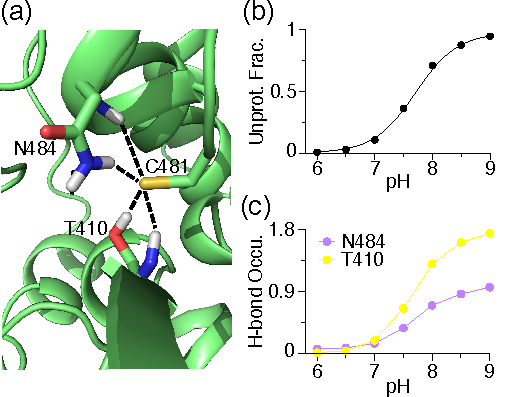
\includegraphics[width=3.3in]{figs/analysis_example.pdf}
    \caption{\textbf{An example analysis of proton titration of a cysteine and coupling with conformational dynamics.}
    (a) A zoomed-in view of the structural environment of Cys481 in the BTK kinase taken from the trajectory at pH 9. 
    The h-bonds with Asn484$\cdots$Cys481 and Thr410$\cdots$Cys481 are shown. 
    The pH 9 replica is used. 
    (b) The unprotonated fractions of Cys481 at different pH conditions. The titration curve represents the best fit to the Henderson-Hasselbalch equation. 
    (c) Occupancy of the h-bond formation between Cys481 thiolate and Asn484 or Thr410
    at different pH conditions. 
  Reprinted with permission from Liu, Zhan et al.\cite{Liu_Shen_2021_J.Med.Chem.} 
    Copyright {2021} American Chemical Society.
    }
\label{Fig:analysis}
\end{figure}
 %--------------------------------------------- 
 



